%%%%%%%%%%%%%%%%%% Automated attack generation %%%%%%%%%%%%%%%%%%%%%%%%%%% (Yu)

%%%%%%%%% Definition of FDIA and cite papers for relevant results
In this section, a generative model is developed for generating successful \textcolor{blue}{FDIAs} targeting the model in (\ref{equ:physical_model}). Including attack signals in the CPS model in \eqref{equ:physical_model} yields the adversarial measurement model
\begin{align}\label{equ:adversarial_measurement_model}
    \mathbf{y}_{I} = H_0\mathbf{x}_{i-T} + H_1\mathbf{u}_{I-1} + \mathbf{e}_{I},
\end{align}
where $\mathbf{e}_{I} = \left[\begin{array}{cccc}\mathbf{e}_{i-T+1}^\top&\mathbf{e}_{i-T+2}^\top&\hdots&\mathbf{e}_i^\top\end{array}\right]^\top$ contains the attack vectors within the moving window $[i-T+1,\hspace{2mm} i]$. Consequently, substituting \eqref{equ:adversarial_measurement_model} into \eqref{equ:state_estimate} yields
\begin{align}\nonumber
    \hat{\mathbf{x}}_i &= A^T\mathbf{x}_{i-T} + F\mathbf{u}_{I-1} + A^T H_0^\dagger\mathbf{e}_{I}\\
    &= \mathbf{x}_i + A^TH_0^\dagger\mathbf{e}_{I}.
\end{align}
Thus, the instantaneous estimation error is given by
\begin{align}\nonumber
    \tilde{\mathbf{x}}_i &= \hat{\mathbf{x}}_i - \mathbf{x}_i\\
    &=A^TH_0^\dagger\mathbf{e}_{I}.
\end{align}
In general, attackers aim to achieve maximum perturbation of certain critical system output without triggering an alarm from the bad data detection mechanism. For this paper, a residual-based bad data detection scheme is used. Let
\begin{align}\label{equ:residual}
    \mathbf{r}_{I} \triangleq \mathbf{y}_{I}-H_1\mathbf{u}_{I-1} - H_0\mathbf{z},
\end{align}
where $\mathbf{z}$ is given in \eqref{equ:RHE}, be the residual vector associated with the receding horizon estimator in \eqref{equ:state_estimate}. Given a threshold value $\tau\in\mathbb{R}$, the bad data indicator for the windowed measurement history is given by
\begin{align}
    \textsf{BDD}(\mathbf{y}_{I}) = \left\{\begin{array}{cl}0&\text{ if }\left\|\mathbf{r}_i\right\|\le\tau\\1&\text{ otherwise.}\end{array}\right.
\end{align}
Substituting \eqref{equ:RHE} and \eqref{equ:adversarial_measurement_model} into \eqref{equ:residual} yields
\begin{align}\nonumber \label{equ:M1}
    \mathbf{r}_{I} &= \left(I-H_0H_0^\dagger\right)\left(\mathbf{y}_{I}-H_1\mathbf{u}_{I-1}\right)\\
    &=\left(I-H_0H_0^\dagger\right)\left(H_0\mathbf{x}_{i-T}+\mathbf{e}_{I}\right).
\end{align}
Thus, from the attacker's perspective, it is desirable to keep the quantity $\left\|\left(I-H_0H_0^\dagger\right)\mathbf{e}_{I}\right\|_2$ as small as possible. 

Next, let $\mathbf{y}_c = C_c\mathbf{x}$ be a vector of critical  output targeted by the attacker. We remark that this is not an attempt to identify a priori the particular outputs targeted by an attacker. Rather, we postulate that there are critical functional outputs which the resilient system designer desires to protect against adversarial targeting. Thus, we define \textcolor{blue}{FDIAs} which target those \textcolor{blue}{outputs} specifically so that the resulting resilient observer can offer the desired protection. \textcolor{blue}{In addition, since most of existing attack generation approaches \cite{zheng2021Resilient, liu2011false} consider the deviation on state estimates as the attack effectiveness, the associated control law is often omitted in the attack generation problem. However, from the development above, it is necessary to consider the controller since the trajectory of the critical output vector $\mathbf{y}_c$ is also affected by the control law which is also affected by the compromised measurements.} Substituting the control law in \eqref{equ:controller} into the linear model in \eqref{equ:physical_model} yields the closed loop system
\begin{align}\nonumber
    \mathbf{x}_{i+1} &= \Bar{A}\mathbf{x}_i + \Bar{B}\tilde{\mathbf{x}}_i,\\
    &=\Bar{A}\mathbf{x}_i + \Bar{B}A^TH_0^\dagger\mathbf{e}_{I}.
\end{align}
where $\Bar{A} = A+BK_p$ and $\Bar{B} = BK_p$. Therefore,
\begin{align}\label{equ:M2}
    \mathbf{y}_{c_{i+1}} = C_c\Bar{A}\mathbf{x}_i + C_c\Bar{B}A^TH_0^\dagger\mathbf{e}_{I}.
\end{align}
Thus, from the attacker perspective, it is desirable to keep the quantity $\left\|C_c\Bar{B}A^TH_0^\dagger\mathbf{e}_{I}\right\|_2$ as big as possible.

We now have all the ingredients to formally define and synthesize the generative model for successful \textcolor{blue}{FDIAs} in CPSs.

\begin{definition}[\textcolor{blue}{($\alpha,\epsilon$)-}Successful \textcolor{blue}{FDIA}]\label{Def:Successful_FDIA}
Consider the CPS in \eqref{equ:physical_model}. Given a positive integer $k<m$, the attack sequence $\mathbf{e}_I \in \Sigma_k \subset \mathbb{R}^{(T+1)m}$, is said to be $(\epsilon, \alpha)$-successful if
\begin{equation}\label{equ:def_success_FDIA}
     \left\|C_c\Bar{B}A^TH_0^\dagger\mathbf{e}_I\right\|_2 \geq \alpha \text{ and }  \left\|\left(I-H_0H_0^\dagger\right)\mathbf{e}_I\right\|_2 \leq \epsilon.
\end{equation}
\textcolor{blue}{for some $\alpha, \epsilon \in \mathbb{R}_{+}$.}
\end{definition}
\begin{remark}
\textcolor{blue}{The first criterion above requires the effectiveness to be at least $\alpha$, while the second criterion guarantees the stealthiness of the attack. Earlier researches formulated the attack generation problem as an effectiveness maximization problem with the stealthiness constraint \cite{liu2011false,mo2010false}. However, this limits the development of attack generators and its application range. Thus, feasibility-based definitions, as above, are currently favored by researchers \cite{sui2020vulnerability}. }
\end{remark}
\noindent In the above definition, $k$ quantifies the attack sparsity level per time. Specifically, it is the maximum number of attacks allowed at each time index. Examples of such successful \textcolor{blue}{FDIAs} can be found in literature; a physics-based \textcolor{blue}{FDIA} generator capable of fooling $\ell_2$ observer, such as Kalman filer, can be found in \cite{mo2010false} and an optimization-based \textcolor{blue}{FDIA} generator capable of fooling stronger $\ell_1$ observer was proposed in \cite{zheng2021Resilient}. However, these \textcolor{blue}{FDIA}s are either computationally too expensive or too conservative to implement on fast real-time systems. In order to circumvent these limitations, we drew inspiration from the \textcolor{blue}{well-known} generative adversarial networks (GAN) \cite{goodfellow2014generative} to build \textcolor{blue}{generative} models for the elements of the set specified by inequalities in \eqref{equ:def_success_FDIA}. 
%%%%%%%% Connect: use (GM) to solve FDIA problem
The Definition~\ref{Def:Successful_FDIA} defines a target set of successful attack signals of the form: 
\begin{equation}\label{equ:success_FDIA_set}
\mathcal{S}(\alpha,\epsilon) \triangleq \big\{\mathbf{e} \hspace{1mm}|\hspace{1mm} \|M_1\mathbf{e}\|_2 \geq \alpha, \|M_2\mathbf{e}\|_2 \leq \epsilon \big\}.
\end{equation}
Thus, the goal of \textcolor{blue}{the} generative model is to learn how to generate elements of that set. 
\begin{definition}
Given a set $\mathcal{S}\subset \mathbb{R}^n$ and a prior distribution $P_z(\mathbf{z})$, a generative model is a mapping of the form $f:\mathbf{z}\mapsto\mathbb{R}^n$ such that $f(\mathbf{z})\in\mathcal{S}$ \textcolor{blue}{with high probability}.
\end{definition}
We consider a generative model of the form $G(\mathbf{z};\boldsymbol{\theta}_g)$, where $\boldsymbol{\theta}_g$ is a tunable parameter vector that will be prescribed to maximize the likelihood of generating elements in $\mathcal{S}$. Specifically, $G$ is taken as a neural network whose input is a random number $\mathbf{z}$ sampled from a prior distribution $P_z$, with weights and biases contained in $\boldsymbol{\theta}_g$. Next, similarly to the GAN framework, $G(\mathbf{z};\boldsymbol{\theta}_g)$ is trained using a fixed discriminator defined by the boundary functions $\|M_1\mathbf{e}\|_2$ and $\|M_2\mathbf{e}\|_2$ of $\mathcal{S}$.

\begin{figure}[h!]
    \centering
    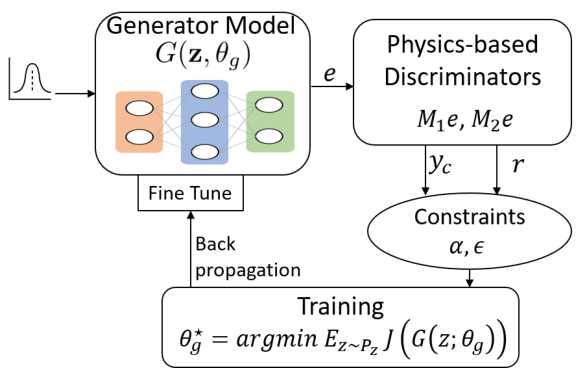
\includegraphics[scale=0.5]{image/GM.png}
    \caption{\textcolor{blue}{Physics-based generative model and training process ($\alpha$ is the lower-bound constraint for attack effectiveness while $\epsilon$ is the upper-bound constraint for attack stealthiness)}}
    \label{fig:GM}
\end{figure}
%%%%%%%% Use Generative model (GM) to generate elements of a set (Mathematical development)
The training process is shown in Fig.~\ref{fig:GM}. The output of the generator is passed, through the discriminator boundary functions, to a loss  function designed such that the weights of the generator network are trained to ensure that the outputs of the discriminators satisfy the constraints. Since the constraints are threshold-based, we use an indicator-like loss function:
\begin{equation}
    J(\mathbf{e}) = \textsf{ReLU}(\alpha - \|M_1\mathbf{e}\|_2)+\textsf{ReLU}(\|M_2\mathbf{e}\|_2 - \epsilon).
\end{equation}

Consequently, the generator is trained by solving the unconstrained optimization problem
\begin{align}\label{equ:training_GM}
    \boldsymbol{\theta}_g^* = \argmin\underset{\mathbf{z}\sim \textbf{P}_z}{\mathbb{E}}J(G(\mathbf{z};\boldsymbol{\theta}_g))
\end{align}
via back propagation.

\iffalse
{\color{red}\textbf{Please update Fig. 1 to reflect the description above. Specifically, replace the Loss Fun with the optimization problem above. Change "Loss Fun" to "training"}}
\fi





